\documentclass[11pt]{book}
\usepackage{amsmath}
\usepackage[russian]{babel}
\usepackage{color}
\usepackage{fullpage}
\usepackage[utf8]{inputenc}
\usepackage{graphicx}
\usepackage{listings}

% for nice symbols
\usepackage{amssymb}
\usepackage{textcomp}
\usepackage{wasysym}
\usepackage{marvosym}

\title{
\small{\textleaf}
\huge{\textleaf}
\huge{\quad}
\large{Сказ о том, чем компилятор от интерпретатора отличается :)}
\huge{\quad}
\huge{\textleaf}
\small{\textleaf}
}
\author{
\small{\textborn} \ 
\small{\APLstar} \ 
\huge{\textborn} \ 
\huge{\APLstar} \ 
\Huge{$\bigstar$} \ 
\huge{\APLstar} \ 
\huge{\textborn} \ 
\small{\APLstar} \ 
\small{\textborn}
\\
\Large (в вольном изложении братца)
\\
\huge{\Bicycle}
}
\date{май 2014}

\begin{document}

\maketitle
\pagebreak

\section*{О чём это}
Программирование сильно смахивает на героическую борьбу человека с компьютером.
Человек пишет программу. Он пишет её на странном, нелогичном языке, с трудом выражая
свои мысли. Язык больше мешает, чем помогает: нужной функции нет, зато есть
куча каких-то дурацких никому не нужных штук.
\\ \\
Вот человек написал программу. Посидел, порассматривал своё кривоватое детище.
С виду --- странная смесь английских слов и бессмысленных крикрзябликов.
Но цепкие глаза программиста смотрят сквозь буквы, въедаются
в неуловимую суть. Наконец человек устаёт пыриться в экран и отдаёт программу
на суд компьютера. Начинается долгое, утомительное противостояние: человек
то букву добавит, то две уберёт, то вообще начинает удалять текст большими кусками.
\\ \\
И вот наступил великий момент: программа запустилась. На чёрном фоне
высветились белые буквы ``Segmentation fault''.
\\ \\
Если ты когда-нибудь будешь программировать (а ты сто пудов будешь ;)), то тебе
тоже в основном придётся сражаться с языком. Причём чем дальше, тем хуже: маленькие
программы пишутся красиво и легко, но как только ты столкнёшься с большой программой,
любой язык подведёт тебя. Одни языки отвалятся сразу. Другие заманят тебя на полпути,
а потом покажут фигу в кармане. Третьи со скрипом, но всё-таки позволят написать на них
заветную программу. Но даже самые лучшие из языков будут регулярно доводить тебя до
нервных припадков.
\\ \\
При этом вокруг будут люди, и все они будут наперебой орать и с пеной у рта
доказывать, что ты выбрала плохой язык. Мол, на их любимом языке программирования
твою программу написать --- раз плюнуть. Некоторые из этих советов --- правда,
некоторые --- нет. Ты никогда не узнаешь этого из разговоров. Ты не узнаешь этого
даже из интересных статей и цветных диаграмм. Единственный способ узнать хоть кусок
настоящей правды --- проверить самому. Серьёзно, не верь, когда кто-то говорит, что
один язык лучше другого. Выслушай все доводы, прими к сведению, сопоставь со своим
опытом. Но никогда не верь слепо и бездумно.
\\ \\
Людям приятнее разводить сотни комментариев на форумах, чем набросать программу на пять
строк и узнать правду. Люди часто не хотят знать правду, потому что это пошатнёт
их мир. Типичный программистский спор сводится к забрасыванию собеседника глупыми
словами, точного значения которых никто не знает. Всё это --- пустой трёп. :\textbackslash
\\ \\
Я хочу, чтоб у тебя было представление о языках в целом: какие они бывают, чем
отличаются, для каких задач подходят. Чтоб у тебя в голове было чёткое представлние,
почему ты делаешь что-то так, а не иначе. Я начну с того, как работает компьютер, потому что
без этого всё остальное --- отвязанная от жизни болтовня. Потом я расскажу,
как от машинного языка можно перейти к языкам высокого уровня. Потом
попытаюсь рассказать про ключевые вещи в языках программирования.
\\ \\
Многие мысли взяты из нескольких умных книжек, и от этих книжек, понятное дело,
больше пользы, чем от одной моей PDF-ки. Если будет время, прочитай их, хотя
бы начало каждой из них. :)
\begin{itemize}
\item Petzold: ``Code''. В этой книжке рассказывается, как вручную собрать
компьютер. Она простая и наполовину состоит из шуток. Если бы из всех книжек
про компы надо было оставить только одну, я б оставила её.
\item Aho, Lam, Sethi, Ullman: ``Compilers: Principles, Techniques, and Tools'' --- книжка про построение
компиляторов. Прочитай первые две главы: первая глава вкратце рассказывает в целом о языках и трансляторах,
а во второй строится маленький компилятор. Эта книжка вообще-то считается
стандартом среди литературы про компиляторы.
\item Jacobs, Grune: ``Parsing Techniques. A Practical Guide'' (2nd edition) --- моя лично горячо любимая книжка про синтаксический анализ.
Там рассказывается про математическую теорию, которая позволяет текст на каком-то языке
структурировать в соответствии с грамматикой этого языка (т.е. ``парсить''). Штука в том,
что почти любой программист вынужден всё время писать парсеры, и лучше чётко представлять себе
ограничения и беды, которые тебя подстерегают. Прочитай оглавление и первые три главы: в первой
и второй главах рассказывается про языки и грамматики, а в третьей проводится обзор
методов грамматического разбора. Это книжка невероятной широты.
\item Kline: ``Mathematics: the Loss of Certainty'' --- про историю математики.
Если ты будешь читать всякие интересные статьи и диссертации, то тебе будут всё чаще
встречаться упоминания интуиниционистской логики, гиперчисел, теоремы Гёделя о неполноте
и прочих странных, ускользающих штук. И если когда-нибудь тебя замучает отсутствие
связности в голове, то эта книжка --- самое оно. Это тоже книжка невероятной широты.
\end{itemize}

\tableofcontents

\chapter{Как устроен компьютер}
Допустим, ты решишь написать программу, которая умножает два числа,
введённых пользователем с клавиатуры, а потом исполнить её на компьютере.
Скорее всего, ты будешь действовать примерно так:
\begin{enumerate}
\item включишь компьютер
\item запустишь Microsoft Visual Studio
\item создашь новый проект типа Console Application
\item добавишь в проект файл main.cpp
\item в файле main.cpp наберёшь текст:
\item{
\begin{verbatim}
    #include <iostream>

    int main ()
    {
        int a;
        int b;

        std::cout << "Enter a:" << std::endl;
        std::cin >> a;
        std::cout << "Enter b:" << std::endl;
        std::cin >> b;
        std::cout << "a * b = " << a * b << std::endl;

        return 0;
    }
\end{verbatim}}
\item Нажмёшь на зелёный треугольник: выскочит чёрное окошко
    с приглашением ввести первое число.
\end{enumerate}
Потом ты задумаешься: а что собственно происходит при
нажатии на зелёный треугольник? Ответ на этот вопрос
примерно такой:
\begin{enumerate}
\item Компиляция.
\\
    Visual Studio запускает встроенный в неё компилятор C++ и передаёт
    ему в качестве аргумента файл main.cpp. Компилятор преобразует код
    на языке C++ в файле main.cpp в код на машинном языке, и сохраняет
    его в новый файл (например main.o). Такой файл с машинными кодами
    называется \emph{объектным} файлом (отсюда и расширение .o).
\item Линковка.
\\
    Каждый .cpp файл преобразуется компилятором в отдельный объектный файл.
    Сами по себе объектные файлы не самодостаточные:
    в одном из них могут использоваться функции, определённые в другом.
    Поэтому объектные файлы нужно объединить в один, и настроить связи
    между ними. Этим занимается линкер.
\\
    Кстати, наш файл main.o тоже не самодостаточный, он использует
    библиотечные функции для ввода-вывода.
\item Исполнение.
\\
    После линковки получается один большой \emph{исполняемый} файл (main.exe).
    Чтобы машинный код в файле main.exe начал исполняться на процессоре,
    нужно во-первых загрузить его в оперативную память, а во-вторых
    указать процессору, с какого адреса в памяти начинать исполнять инструкции
    (то есть передать управление на начало этого кода). Этим занимается загрузчик.
\end{enumerate}
В этом объяснении многое остаётся непонятным. Наверное,
самое непонятное, это ``машинный код''. Чем он так сильно отличается
от другого кода, что вдруг становится понятным процессору?
Другая странность --- это тайная связь оперативной памяти и процессора.
Почему-то, чтобы процессор начал исполнять машинный код, надо загрузить
этот код в оперативную память. А где он был до этого? И что значит
``указать процессору, с какого адреса в памяти начинать исполнять
инструкции''?
\\ \\
Чтобы это понять, надо представлять, как устроен компьютер. В общем,
есть четыре основных компонента, без которых ну никак:
\begin{enumerate}
\item процессор
\item память
\item устройство ввода
\item устройство вывода
\end{enumerate}
У процессора две главных функции: выполнять арифметико-логические операции
(складывать, умножать, сравнивать и т.д.), и задавать темп работы
(отсчитывать такты). Память, нужна чтобы хранить в ней что-то, иначе всё, что насчитал
процессор, потеряется. Ну и наконец, без устройств ввода/вывода с компьютером вообще ничего нельзя
сделать.
\\ \\
Такое объяснение не противоречит здравому смыслу, но и только. Оно слишком
общее, чтобы понять, что такое машинный код и как исполняются программы.
Кроме того, непонятно, почему компьютер должен быть
устроен именно так: то-ли по законам природы, то-ли по чудовищной случайности.
Поэтому щас я попытаюсь пошагово построить компьютер: начну с
необходимого минимума и буду постепенно добавлять элементы,
которые не сделаешь на основе тех, что уже есть.

\section{Физическая основа}
Компьютер придумали для автоматизации вычислений. Автоматизация
вычислений произошла по четырём причинам:
\begin{enumerate}
\item люди считают медленно
\item люди допускают ошибки
\item людям лень считать
\item люди невероятно умные
\end{enumerate}
Поэтому естественная для человека мысль --- использовать какой-то
физический процесс для своих целей. Можно сплавлять брёвна вниз по реке.
Можно построить водяную или ветряную мельницу. Можно сделать песочные часы.
\\ \\
В основе компьютера тоже должен лежать какой-то физический процесс,
и сейчас это электричество. Но надо понимать, что чисто теоретически вместо
электричества может быть что угодно (и было: первые компьютеры были механические,
а в последнее время некоторые пытаются построить компьютер на основе какого-то
хитрого вида плесени).
\\ \\
С другой стороны, надо понимать, что электричество в компьютерах не случайно:
оно во многом \emph{позволило} сделать компьютер. Механический компьютер
той же сложности, что твой ноут, был бы невменяемого размера.
Все процессы шли бы в нём крайне медленно (пока шестерёнки с одного
конца докрутятся до другого). Кроме того, детали в этом компе ломались бы так часто,
что комп был бы всё время сломан.

\subsection{Электрические схемы и логика}
Начнём с простой схемы:
\\
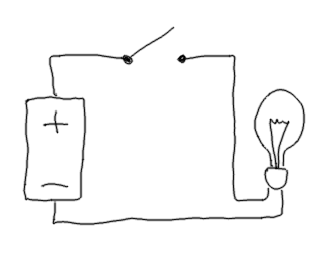
\includegraphics[height=1in]{pic/2.png}
\\
В этой цепи немного элементов: лампочка, батарея, ключ. Если ключ разомкнут,
ток не идёт, и лампочка не горит. Если ключ замкнут, ток идёт, и лампочка горит.
Кстати, лампочка нас интересует только как индикатор, есть ток или нет.
В целом зависимость ``лампочка - ключ'' можно охарактеризовать таблицей:
\\
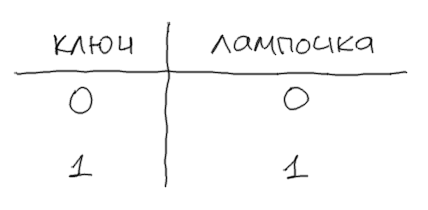
\includegraphics[height=1in]{pic/3.png}
\\
Таблицы такого рода, задающие зависимость истинности/ложности одних переменных
от истинности/ложности других переменных, называются \emph{таблицами истинности} или \emph{таблицами логики}.
Добавим ещё один ключ в схему (последовательно):
\\
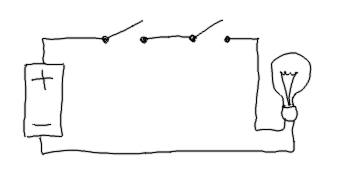
\includegraphics[height=1in]{pic/4.png}
\\
Теперь лампочка зависит от двух ключей: она горит, только если первый
\emph{и} второй ключ замкнут. Вот соответствующая таблица логики:
\\
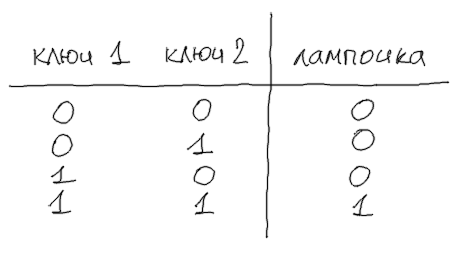
\includegraphics[height=1.5in]{pic/5.png}
\\
Если бы мы добавили второй ключ параллельно, схема бы получилась такой:
\\
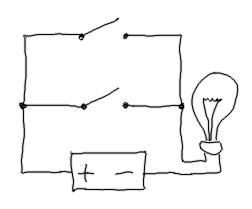
\includegraphics[height=1.5in]{pic/6.png}
\\
В этой схеме лампочка горит, только если первый \emph{или} второй ключ замкнут.
Вот её таблица логики:
\\
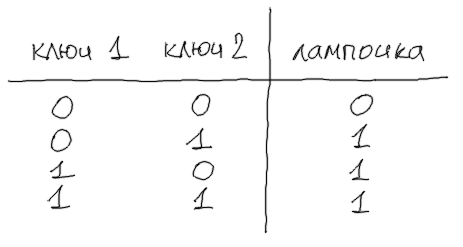
\includegraphics[height=1.5in]{pic/7.png}
\\
Мы получили две интересных схемы: первая отражает логическое \emph{и} (AND), вторая ---
логическое \emph{или} (OR). На основе этих схем можно собирать другие, более сложные.
Например, есть у тебя условие: ``если я сдам лабу или будет солнечно,
то я пойду гулять''. Это условие описывается схемой OR:
\\
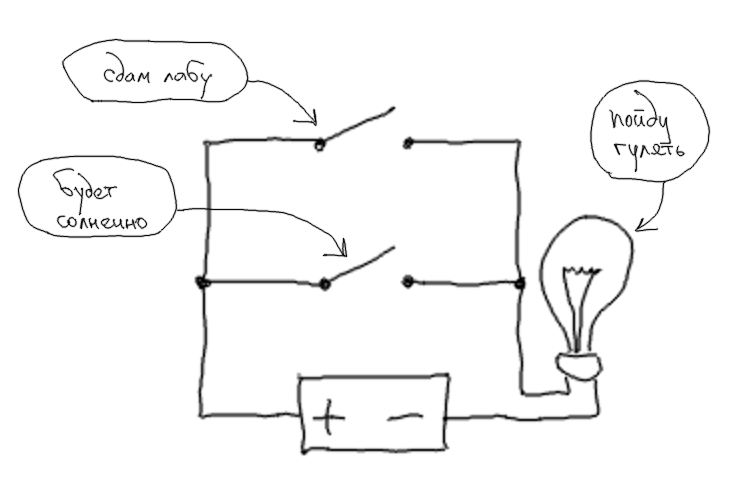
\includegraphics[height=2in]{pic/8.png}
\\
Преподаватель, которому ты собралась сдавать лабу, знает, что если у него
будет хорошее настроение, то ты сдашь лабу. Его настроение зависит от двух вещей:
во-первых, будет ли солнечно, а во вторых, успеет ли он пообедать.
Он может описать это с помощью схемы AND:
\\
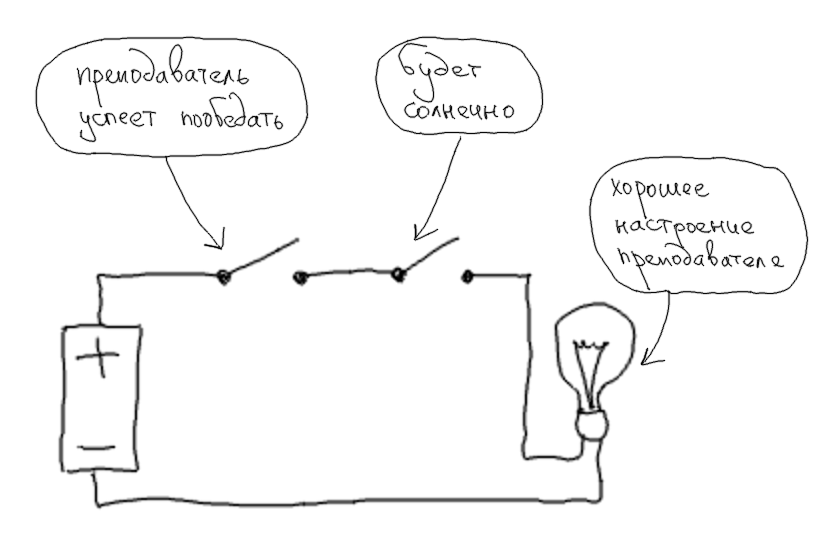
\includegraphics[height=2in]{pic/9.png}
\\
Допустим, преподаватель хочет узнать, пойдёшь ли ты завтра гулять, но не очень
хорошо разбирается в хитросплетениях твоей логики. Зато у него есть твоя схема.
Он берёт её и пытается присобачить к ней свою. Логически это очень просто:
нужно связать выход ``хорошее настроение'' со входом ``сдам лабу'': если на выходе
``хорошее настроение'' есть ток, ключ ``сдам лабу'' замкнут, если тока нет --
разомкнут:
\\
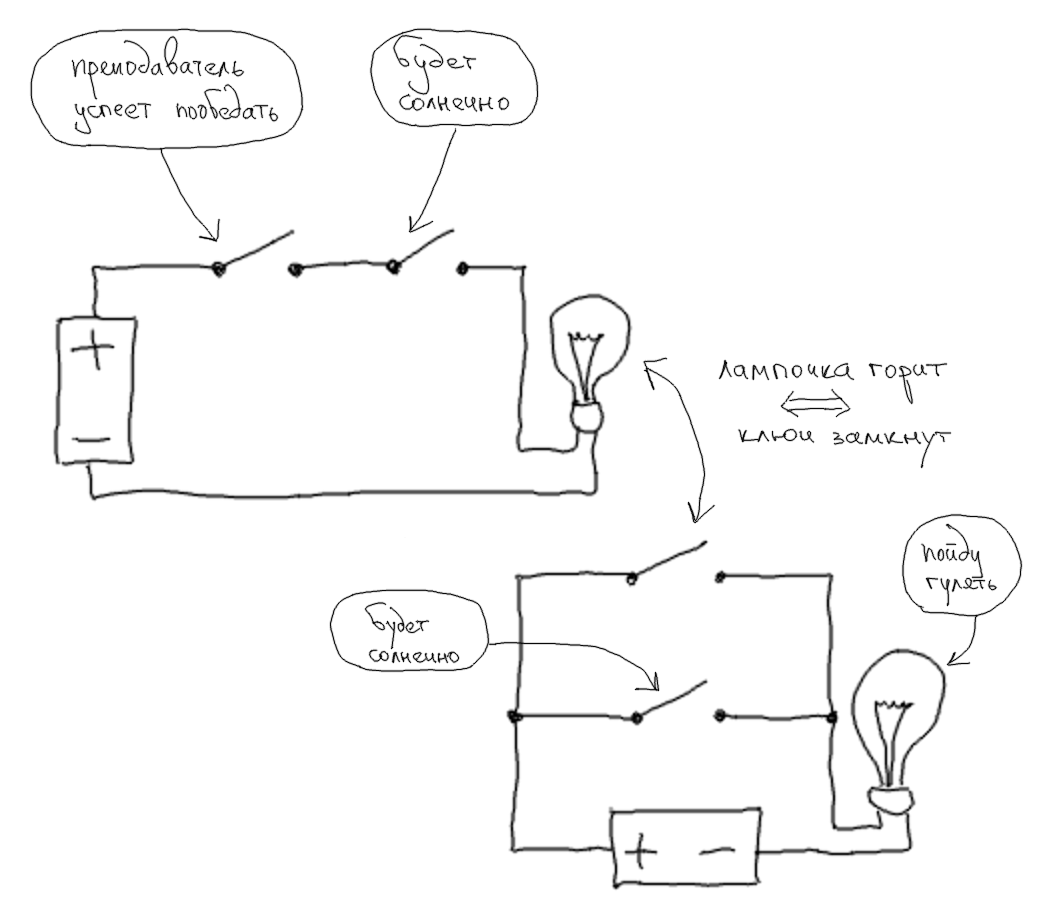
\includegraphics[height=3.5in]{pic/10.png}
\\
Поначалу можно вручную замыкать и размыкать ключ, но это быстро надоест
(особенно когда схема станет большой). Нужно что-то, что само замыкало и
размыкало бы ключ в зависимости от тока. Одним из таких устройств является
реле:
\\
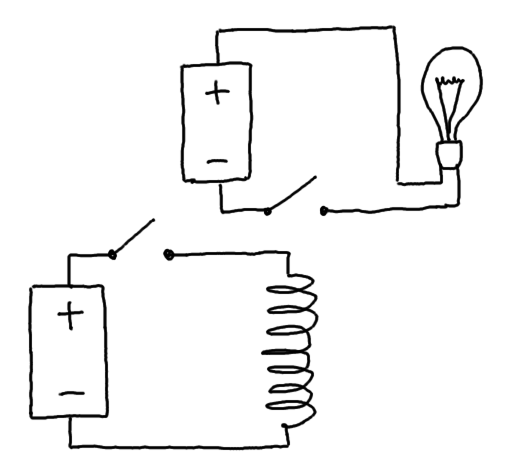
\includegraphics[height=2in]{pic/11.png}
\\
Если в первой цепи течёт ток, то катушка намагничивается и начинает притягивать
ключ во второй цепи. Ключ замыкается. Если в первой цепи ток пропадает, то катушка размагничивается,
перестаёт притягивать ключ и он размыкается. Реле позволяет связать вход
``сдам лабу'' с выходом ``хорошее настроение'':
\\
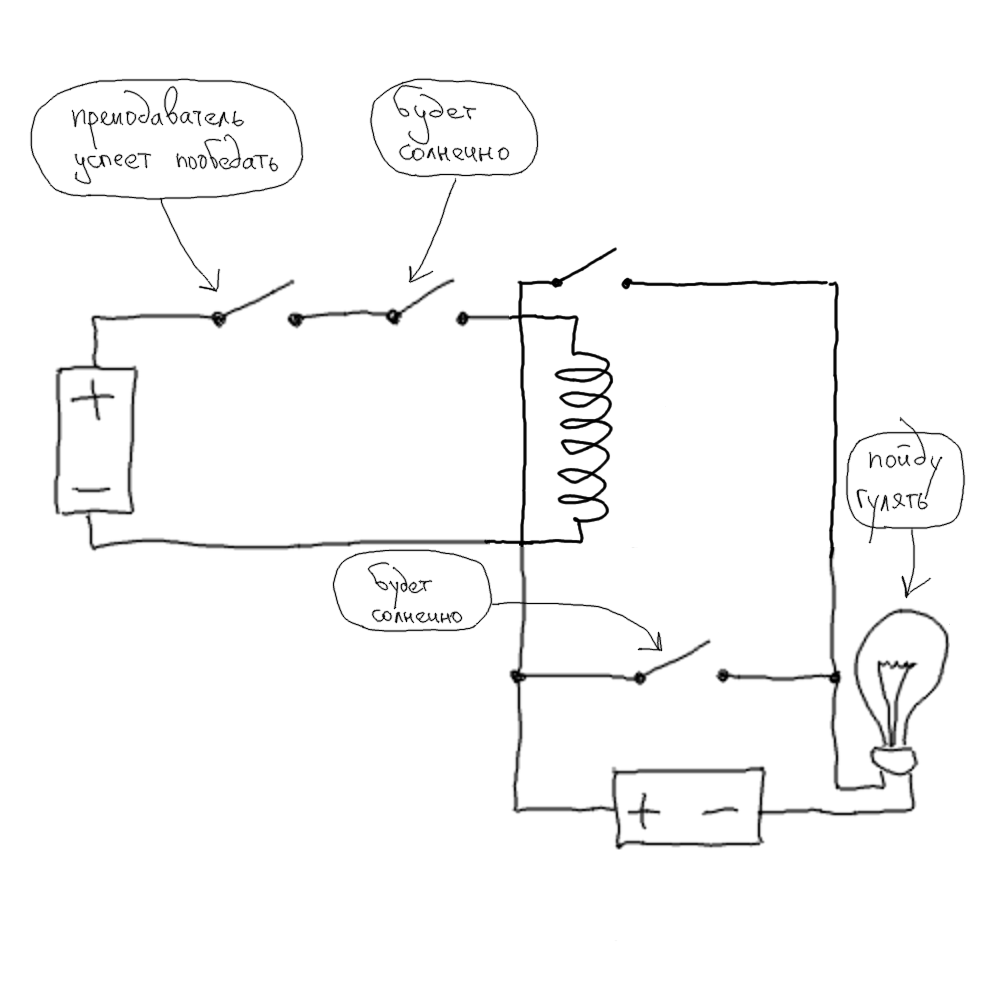
\includegraphics[height=3.5in]{pic/12.png}
\\
Конечно, эту конкретную схему можно упростить и выкинуть реле, просто встроив преподавательскую схему
в твою вместо ключа ``сдам лабу'':
\\
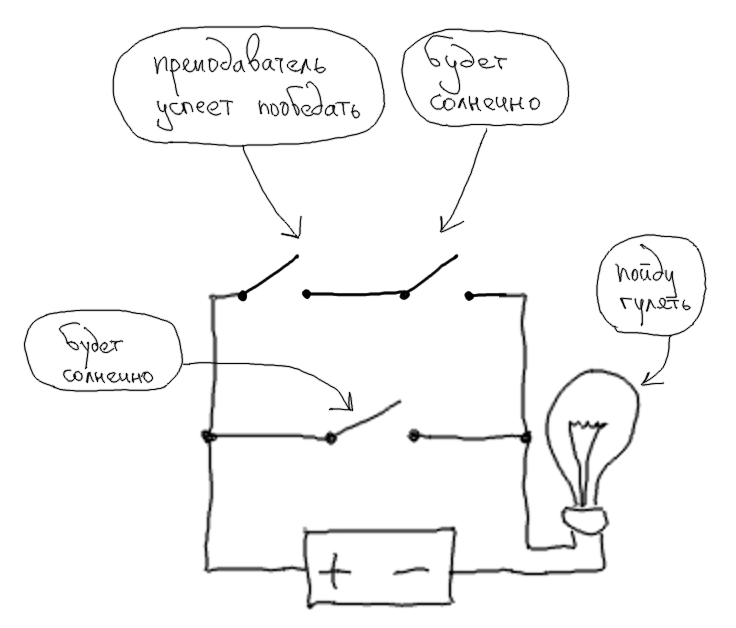
\includegraphics[height=3.5in]{pic/13.png}
\\
И даже ещё сильнее упростить:
\\
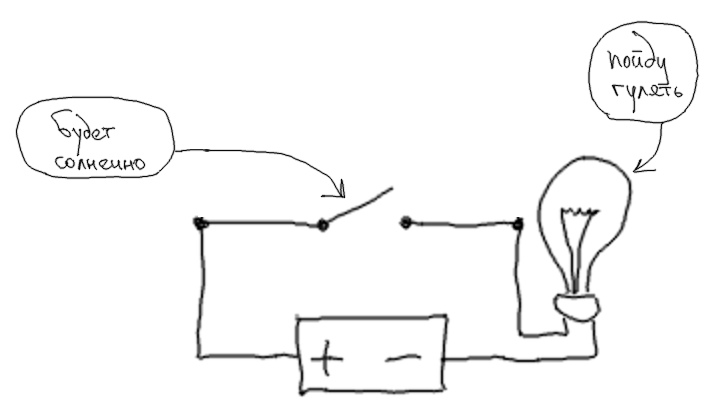
\includegraphics[height=2in]{pic/14.png}
\\
Но упростить не всегда возможно и никогда не поздно, и пусть этим занимаются разработчики микросхем.
Мне важно показать, что схему в принципе \emph{можно} собрать. Реле позволяет нам управлять входом схемы при помощи наличия/отсутствия тока,
а не при помощи замыкания/размыкания ключа. А наличие/отсутствие тока --- это как раз то,
что является выходом любой схемы. Поэтому можно сделать очень
важное предположение: что любой выход одной схемы можно соединить с любым входом другой
схемы. (Кстати, реле полезно не только для связывания разных схем, а ещё и просто как повторитель, для усиления слабого тока.
Именно для передачи сигнала на большие расстояния реле использовалось в телеграфных линиях.)
\\ \\
Реле --- не единственное устройство, способное замыкать и размыкать ключ
в зависимости от тока (но первое, которое применили в компьютерах). Сейчас
используются транзисторы, а до этого были вакуумные лампы.
\\ \\
Вот как выглядят схемы AND и OR с использованием реле:
\\
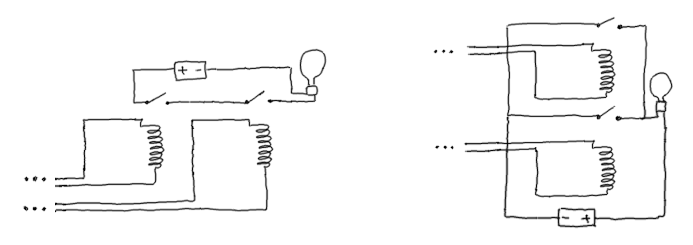
\includegraphics[height=2in]{pic/15.png}
\\
Строго говоря, это уже не схемы, а фрагменты схем. Но, с другой стороны, ``выход'' схемы ---
тоже не выход, а кусок цепи, по которому идёт или не идёт ток. Чтобы соединить выход
и фрагмент, нужно разомкнуть цепь в районе выхода и получившиеся два конца провода примотать
к концам провода, торчащим из фрагмента:
\\
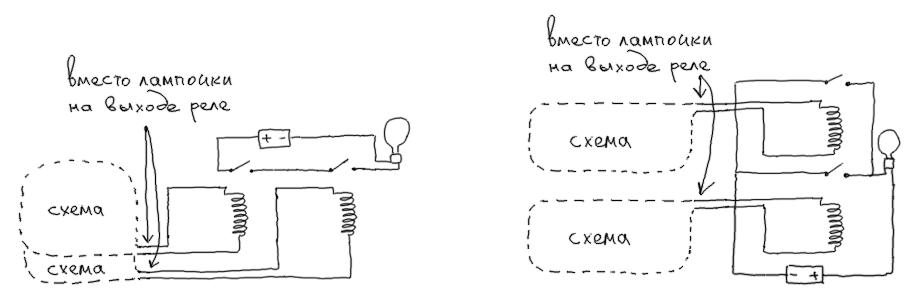
\includegraphics[height=2in]{pic/16.png}
\\
Дальше я всё буду называть схемой. Вот ещё одна важная схема, отражающая ``логическое \emph{не}'', NOT:
\\
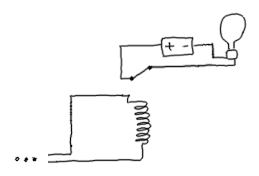
\includegraphics[height=1.5in]{pic/17.png}
\\
В предыдущих схемах реле повторяло сигнал, а здесь оно его инвертирует: если в первой цепи идёт ток, то во второй тока нет, и наоборот.
Поэтому схема называется \emph{инвертором}.
\\ \\
Оказывается, что вместе три эти простенькие схемы --- И, ИЛИ, НЕ --- обладают невероятной силой.
С помощью них можно собрать ЛЮБУЮ логическую схему! (И это ещё не всё: из схем И и НЕ можно
собрать схему ИЛИ, а из схем ИЛИ и НЕ можно собрать схему И. Есть вообще такие схемы И-НЕ и ИЛИ-НЕ,
что с помощью каждой из них (одной) можно собрать все остальные. Дальше по этой
теме читай про ``полные системы булевых функций''.)
\\ \\
Для этих трёх схем --- И, ИЛИ, НЕ --- я введу общепринятые обозначения:
\\ \\
Как видишь, входы и выходы обозначаются одинаково, в виде куска торчащего
провода. Я буду говорить ``подать ток на вход''. Понятно, что с точки зрения физики это
бред, потому что нельзя просто так взять и подать ток куда-то. Но (надеюсь) понятно,
что я имею в виду.
\\ \\
Почти всё дальнейшее построение компьютера сведётся к сборке более сложных схем
из этих трёх.

\subsection{Двоичная система счисления}
Я вот всё время говорю про логические схемы и булевые функции (что по сути одно и то же),
и даже собрала маленькую схему для определения, пойдёшь ли ты гулять. Более того, я собрала
несколько простых схем (И, ИЛИ, НЕ) и говорю, что с их помощью можно собрать
любую логическую схему. В смысле логических схем наще будущее явно обеспечено.
Но всё-таки, какая ИМЕННО от них польза?
\\ \\
Пока понятно только, что электричество удивительно хорошо для них подходит.
В электричестве есть два чётких состояния: есть ток, нет тока. И в логике
есть два элемента: правда, ложь. Если б мы захотели с помощью электричества моделировать
социальные анкеты (``да'', ``нет'', ``не знаю''), нам пришлось бы выдумывать, как обозначать
третий элемент (например, есть ток, но слабый). Тем более тяжело было бы
с десятичными цифрами.
\\ \\
А мы-то как раз с цифрами (вернее, с числами) работать и собрались, потому что
что это за компьютер, который даже два числа сложить не может. К счастью, нам не
придётся моделировать десять состояний (в отличие от тех, кто строил первые
компьютеры). Мы просто будем все вычисления внутри компьютера проводить над числами
в двоичном представлении.
\\ \\
Важное замечание: от того, что мы решили использовать в компьютере двоичные,
а не десятичные числа, С ТОЧКИ ЗРЕНИЯ ПОЛЬЗОВАТЕЛЯ НИЧЕГО НЕ МЕНЯЕТСЯ: число
это просто абстрактная идея, и не важно, в каком виде она выражена. Компьютер
будет делать ровно то же, что и с десятичными числами: решать такие же задачи
и выдавать такие же результаты. Потом, если угодно, можно сделать специальную приставку,
которая будет позволять вводить/выводить десятичные числа, и переводить их
для компьютера в двоичное представление.

\section{Сумматор}
Итак, компьютер нужен для автоматизации вычислений.
Поэтому первое, без чего не обойдётся ни один компьютер, это устройство
для сложения чисел. Попробуем собрать такое устройство --- сумматор.
\\ \\
Чтобы понять, как должен работать двоичный сумматор, надо
вспомнить, что делает человек, когда складывает двоичные числа.
Сложение происходит поразрядно и с переносом:

\begin{enumerate}
\item
   k = 1
\\
   перенос = 0
\\
   если одно число короче другого, дополнить его нулями в старших разрядах
\\
   N = число разрядов
\\
\item Определяем k-й разряд первого суммы и новый перенос по таблице:
\begin{verbatim}
   -------------------------------------------------------------------
   | k-й разряд    | k-й разряд    | перенос || k-й разряд | перенос |
   | первого числа | второго числа |         || суммы      | (новый) |
   |---------------|---------------|---------||------------|---------|
   |       0       |       0       |    0    ||     0      |    0    |
   |       0       |       0       |    1    ||     1      |    0    |
   |       0       |       1       |    0    ||     1      |    0    |
   |       0       |       1       |    1    ||     0      |    1    |
   |       1       |       0       |    0    ||     1      |    0    |
   |       1       |       0       |    1    ||     0      |    1    |
   |       1       |       1       |    0    ||     0      |    1    |
   |       1       |       1       |    1    ||     1      |    1    |
   -------------------------------------------------------------------
\end{verbatim}
\item k = k + 1
\item если k < N
\\
       перейти к шагу 2
\end{enumerate}


Видимо, главное в этом алгортме --- таблица, по которой определяются новый перенос
и k-й разряд суммы. Без этой таблицы не обойтись: в жизни мы принимаем как аксиому,
что 0+0=0, 0+1=1, 1+0=1, 1+1=0 и 1 в уме. В сумматор тоже придётся встроить эти
правила.
\\ \\
Итак, нам нужна схема, у которой три входа: k-й разряд первого слагаемого,
k-й разряд второго слагаемого и перенос, и два выхода: k-й разряд суммы и перенос
на (k + 1)-й разряд. Отстуствие тока на входе или выходе означает ноль,
наличие --- единицу. Внутри схема должна быть устроена так, чтобы зависимость
выходов от входов была такая же, как в таблице.
\\ \\
Это очень похоже на схемы И, ИЛИ, НЕ, только наша схема более сложная.
Чтобы слегка упростить схему, разобьём её на две полсхемы. Сделать это
можно так: вместо того, чтобы сразу пытаться сложить три входа
(k-й разряд первого числа, k-й разряд второго числа, перенос), будем
два раза складывать по два входа: сначала k-й разряд первого числа и k-й разряд второго числа,
а потом результат первого сложения и перенос.
\\ \\
Когда складываешь два входа, может возникнуть перенос (если оба входа равны 1).
Поэтому у каждой полсхемы будет два входа (для слагаемых) и два выхода
(для суммы и переноса):
\begin{verbatim}
   ----------------------------------------------------
   | 1-е слагаемое | 2-е слагаемое || сумма | перенос |
   |               |               ||       |         |
   |---------------|---------------||-------|---------|
   |       0       |       0       ||     0 |     0   |
   |       0       |       1       ||     1 |     0   |
   |       1       |       0       ||     1 |     0   |
   |       1       |       1       ||     0 |     1   |
   ----------------------------------------------------
\end{verbatim}
Чтобы собрать такую полсхему, снова разобьём её на две четвертьсхемы,
одна для суммы, а вторая для переноса:
\begin{verbatim}
   ------------------------------------------
   | 1-е слагаемое | 2-е слагаемое || сумма |
   |               |               ||       |
   |---------------|---------------||-------|
   |       0       |       0       ||     0 |
   |       0       |       1       ||     1 |
   |       1       |       0       ||     1 |
   |       1       |       1       ||     0 |
   ------------------------------------------
   --------------------------------------------
   | 1-е слагаемое | 2-е слагаемое || перенос |
   |               |               ||         |
   |---------------|---------------||---------|
   |       0       |       0       ||     0   |
   |       0       |       1       ||     0   |
   |       1       |       0       ||     0   |
   |       1       |       1       ||     1   |
   --------------------------------------------
\end{verbatim}

Четвертьсхема для переноса совсем простая --- это попросту схема И.
С суммой всё не так просто, но взяв две схемы ИЛИ, одну схему НЕ и одну схему И,
мы получим то, что надо:
\\ \\
Остаётся объединить входы четвертьсхем для суммы и переноса,
и полсхема для сложения двух входов готова:
\\ \\
Теперь пора связать полсхемы. У первой полсхемы два входа:
k-й разряд первого слагаемого и k-й разряд второго слагаемого.
У второй полсхемы первый вход --- это выход ``сумма'' первой полсхемы,
а второй вход --- перенос:
\\ \\
У нас остался один выход ``сумма'' --- как раз как надо. Но выходов ``перенос'' по прежнему два,
а нужен один. Из-за разбиения сложения на два этапа на каждом этапе получился свой перенос.
Но ведь в жизни всё равно, сразу три числа складывать, или сначала сложить два, а потом прибавить
третье --- результат один и тот же. Что-то тут не то! Если повнимательнее рассмотреть полученную нами схему
с тремя выходами, то её работа описывается такой таблицей логики:
\begin{verbatim}
   -------------------------------------------------------------------------------------
   | k-й разряд    | k-й разряд    | перенос || k-й разряд | 1-й перенос | 2-й перенос |
   | первого числа | второго числа |         || суммы      |             |             |
   |---------------|---------------|---------||------------|-------------|-------------|
   |       0       |       0       |    0    ||     0      |    0        |    0        |
   |       0       |       0       |    1    ||     1      |    0        |    0        |
   |       0       |       1       |    0    ||     1      |    0        |    0        |
   |       0       |       1       |    1    ||     0      |    0        |    1        |
   |       1       |       0       |    0    ||     1      |    0        |    0        |
   |       1       |       0       |    1    ||     0      |    0        |    1        |
   |       1       |       1       |    0    ||     0      |    1        |    0        |
   |       1       |       1       |    1    ||     1      |    1        |    0        |
   -------------------------------------------------------------------------------------
\end{verbatim}

Из таблицы видно, что хотя переноса два, они не бывают одновременно равны 1.
Поэтому их можно объединить при помощи схемы ИЛИ:
\\ \\
Готово! Вот она, чудо-схема для сложения разрядов с переносом.

\section{Команды}
...
\section{Память}
...
\section{Счётчик}
...
\chapter{Переход к языкам высокого уровня}
...
\section{Ассемблер}
...
\section{Необходимость абстрагироваться от машины}
...
\section{Языковые процессоры}
...
\subsection{Компиляторы}
...
\subsection{Интерпретаторы}
...
\subsection{JIT-компиляторы}
...
\subsection{Промежуточные представления}
...
\subsection{Виртуальные машины}
...
\subsection{Детсадовский пример}
\definecolor{cgray}{rgb}{0.96, 0.95, 0.9}
\definecolor{cblue1}{rgb}{0.0, 0.15, 0.3}
\definecolor{cblue2}{rgb}{0.0, 0.4, 0.6}
\definecolor{cblue3}{rgb}{0.0, 0.7, 1.0}
\definecolor{cgreen}{rgb}{0.2, 0.6, 0.0}
\lstdefinestyle{cxx}
    { numbers=left
    , numberstyle=\footnotesize\ttfamily\color{cblue3}
    , breaklines=true
    , language=C++
    , basicstyle=\footnotesize\ttfamily\color{cblue1}
    , keywordstyle=\footnotesize\ttfamily\color{cblue2}
    , commentstyle=\itshape\color{cgreen}
    , backgroundcolor=\color{cgray}
    }
\lstset{style=cxx}
Теперь возьмём игрушечный язык и построим для него:
\begin{enumerate}
\item Интерпретатор
\item Компилятор
\item Виртуальную машину
\item Интерпретатор байткода виртуальной машины
\item JIT-компилятор байткода виртуальной машины
\end{enumerate}
Все эти программы будут написаны на языке C++.
\\ \\
Первым делом мы построим формальную грамматику для нашего языка и
обсудим некоторые её особенности.
\\ \\
Потом перейдём к построению парсера: выберем алгоритм синтаксического разбора
и немного подпилим грамматику под этот алгоритм. В процессе пояснения алгоритма
мы напишем простенький прототип будущего парсера на языке Haskell с использованием
библиотеки Parsec. Парсер будет преобразовывать программы на нашем языке в
промежуточное представление --- AST, общее для всех языковых процессоров.
В конце главы мы перепишем парсер на C++. Парсер, пожалуй, самая сложная часть
нашего примера.
\\ \\
После этапа синтаксического разбора каждый языковой процессор пойдёт своим путём.
\\ \\
Первым номером мы построим интерпретатор: он будет обходить AST и сразу же выполнять
программу. Интерпретатор будет очень простым.
\\ \\
Вторым номером мы построим компилятор. Мы будем компилировать программу на нашем языке
в машинный код для архитектуры x86-64. В отличие от обычных компиляторов, мы пропустим фазу линковки
и сразу создадим исполняемый файл. В этом файле кроме самой программы будет содержаться
ещё информация для загрузчика. Поскольку формат исполняемого файла зависит от операционной системы,
нам придётся ограничиться конкретной операционной системой --- Linux. Мы сгенерируем
исполняемый файл в формате ELF (для этого нам придётся слегка разобраться в формате ELF).
\\ \\
Потом мы разработаем \emph{стековую} виртуальную машину для нашего
языка и напишем компилятор в байткод этой виртуальной машины. Этот компилятор будет очень простым,
он будет генерировать инструкции для виртуальной машины и сохранять их в буфер.
\\ \\
Потом мы напишем интерпретатор байткода виртуальной машины (он тоже будет очень простым).
\\ \\
Последним номером мы напишем JIT-компилятор байткода виртуальной машины в машинный код для архитектуры x86-64.
В отличие от компилятора, который только генерирует исполняемый файл (но не исполняет его),
JIT-компилятор будет генерировать код и тут же его исполнять, т.е. динамически транслировать код.
Поэтому нам не придётся снова возиться с генерацией исполняемого файла: мы будем просто записывать
инструкции в кусок памяти и передавать на него управление. Однако нам придётся немного повозиться,
чтоб операционная система разрешила вытворять такие безобразия.
\\ \\
Хочу подчеркнуть, что это просто несколько примеров языковых процессоров, и существует много других.
Например, JIT-компилятор вовсе не привязан к байткоду виртуальной машины: он мог бы компилировать
оригинальную программу. Кроме того, ни один из рассмотренных языковых процессоров не проводит
никаких оптимизаций (наш язык слишком простой для них).

\subsubsection{Грамматика}
Язык я выберу очень простой: арифметические операции над целыми числами
в десятичном представлении. Этот язык можно описать такой грамматикой $G=<V,W,P,S>$:

$$V=\{0,1,2,3,4,5,6,7,8,9,+,-,*,/,(,)\}$$
$$W=\{digit, number, factor, term, expr\}$$
$$P=\left\{
\begin{array}{l l}
digit \  & \rightarrow \ 0 \ | \ 1 \ | \ 2 \ | \ 3 \ | \ 4 \ | \ 5 \ | \ 6 \ | \ 7 \ | \ 8 \ | \ 9
\\
number \  & \rightarrow \ digit \ number \ | \ digit
\\
factor \  & \rightarrow \ number \ | \ ( expr )
\\
term \  & \rightarrow \ term * factor \ | \ term / factor \ | \ factor
\\
expr \  & \rightarrow \ expr + term \ | \ expr - term \ | \ term
\end{array}
\right. $$
$$S=expr$$
\\
Эта грамматика может показаться сложноватой.
Во-первых, вместо трёх правил для нетерминалов $factor$, $term$ и $expr$ можно обойтись
одним:
$$expr \  \rightarrow \ expr + expr \ | \ expr - expr \ | \ expr * expr \ | \ expr / expr \ | \ ( expr ) \ | \ number$$
\\
Это правило позволяет описывать те же самые языковые конструкции, что и три правила $factor$, $term$ и $expr$ вместе взятые.
Кроме того, оно проще и очевиднее. Зачем разбивать его на три? А вот зачем:
такое разделение позволяет прямо в грамматике закодировать \emph{приоритеты} арифметических операций.
У скобок самый большой приоритет (правило $factor$); затем идут мультипликативные операции с меньшим приоритетом (правило $term$);
затем аддитивные с ещё меньшим приоритетом (правило $expr$). Получается, что трёхуровневые правила
описывают тот же \emph{синтаксис}, что и одноуровневое, но при этом описывают часть \emph{семантики} языка
(приоритет арифметических операций).
\\ \\
Вторая странность нашей грамматики, это то, что правила для арифметических операций имеют вид
$a \rightarrow a \circ b$. Возьмём, например, правило для сложения:
$expr \rightarrow expr + term$. Почему не $expr \rightarrow term + expr$ ? Или самый очевидный
вариант: $expr \rightarrow expr + expr$ ? Все три варианта описывают синтаксически эквивалентные языковые конструкции.
Чем первый вариант лучше? Дело тут в другой семантической особенности
нашего языка: \emph{левоассоциативность} бинарных операторов вычитания и деления.
Выражение ``$1 - 2 - 3$'', к примеру, следует понимать как ``$(1 - 2) - 3$'', а не ``$1 - (2 - 3)$''.
Рассмотрим повнимательнее правило для вычитания: $expr \rightarrow expr - term$.
Слева от ``$-$'' стоит $expr$, т.е. любое выражение. А вот справа --- $term$,
т.е. выражение, допускающее только мультипликативные операции над числами и выражениями в скобках.
Получается, такое правило заставляет нас однозначно понимать ``$1 - 2 - 3$'' как ``$(1 - 2) - 3$''.
Если бы мы выбрали правило $expr \rightarrow term - expr$, мы бы получили \emph{правоассоциативный}
оператор вычитания (и такие операторы иногда нужны). А вот третье правило, $expr \rightarrow expr - expr$,
вообще \emph{неоднозначное}: оно позволяет понимать выражение ``$1 - 2 - 3$''
двумя способами. Неоднозначность в грамматиках --- источних бед. Её следует допускать только тогда, когда
сам по себе язык неоднозначен (как, например, русская фраза ``он умеет заставить себя слушать'').
Кстати, правила для сложения и умножения могут быть как левоассоциативными, так и правоассоциативными, лишь бы не неоднозначными.
\\ \\
Итак, у нас есть очень хорошая и правильная грамматика: она не только
описывает всевозможные арифметические выражения, но ещё и придаёт им глубоко арифметический
смысл. Правильная грамматика --- это полдела, потому что благодаря ей мы
чётко понимаем, с чем мы имеем дело.

\subsubsection{Парсер}
Раз уж мы собрались строить языковые процессоры для языка арифметических
выражений, то начинать нужно с парсера. Парсер должен структурировать входную
строку в соответствии с нашей грамматикой:
\\ \\
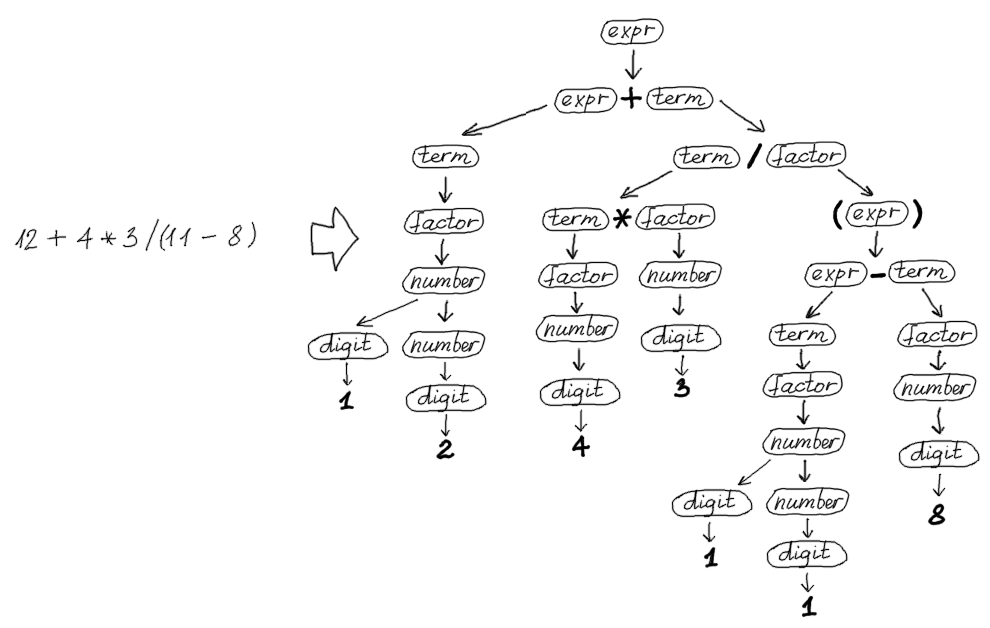
\includegraphics[height=3.5in]{pic/18.png}
\\ \\
Дерево на картинке --- это \emph{дерево разбора}. (Вообще, правильнее было бы
говорить \emph{граф разбора}, потому что он только в простых случаях является деревом. Но термин
``дерево'' как-то прижился). Возникает два вопроса:
\begin{enumerate}
\item Как заставить парсер догадаться, какая стуктура соответствует строке?
Явно придётся выковыривать символы, искать среди них плюсы, минусы и прочее.
Но как сделать это грамотно?
\item Допустим, парсеру каким-то чудом удалось распознать в строке
структуру. Что он должен делать с этим тайным знанием? Немедленно использовать
и тут же забыть? Или как-то сохранить для последующего использования?
\end{enumerate}
Разберёмся сначала с первым.
\\ \\
Один из самых простых подходов при написании парсера --- это так называемый \emph{метод
рекурсивного спуска} (recursive descent). Суть метода такая: для каждого нетерминала пишется
отдельная маленькая функция-парсер. Эта функция вызывает функции-парсеры для других нетерминалов (возможно, саму себя) ---
точно так же, как правила грамматики ссылаются друг на друга. В итоге
парсер структурно повторяет грамматику. Примерно так:

\lstinputlisting[language=Haskell]{example_recursive_descent/parser1_bad.hs}
Парсер написан на языке Haskell с использованием библиотеки Parsec.
Как видно из 1-й строки, мы взяли всего три библиотечных функции: \texttt{<|>}, \texttt{char} и \texttt{parse}.
Остальное --- встроенные хаскельные функции и операторы.
Оператор \texttt{<|>} работает как логическое \emph{или}: запускает левый парсер,
и если он отработал неудачно, запускает правый парсер.
Оператор \texttt{>\thinspace >} работает как логическое \emph{и}: запускает левый парсер,
и если он отработал удачно, запускает правый парсер.
Поскольку наш парсер пока не возвращает никакого результата (только проверяет синтаксическую корректность),
то все функции-парсеры должны возвращать значение типа \texttt{()} 
(аналог типа \texttt{void} в С/С++). Чтобы возвращать \texttt{()},
функция должна конце вызывать \texttt{return ()} или другую функцию, которая возвращает \texttt{()}.
\\ \\
Метод рекурсивного спуска --- это очень простой метод
построения парсеров, наиболее \emph{естественный} для человека: он позволяет писать парсер почти не задумываясь,
просто глядя на грамматику. На практике у этого метода есть две основные проблемы.
\\ \\
Первая проблема --- корректный перебор нескольких альтернатив. Если не сработал первый парсер, надо не просто
запустить второй, но ещё и перед этим аккуратно откатить назад все изменения, сделанные первым (backtrack).
В частности, если первый парсер продвинулся на несколько символов во входной строке,
то надо вернуться на прежнюю позицию. В библиотеке Parsec для этого есть функция \texttt{try}:
она запоминает состояние, к которому нужно откатиться.
С учётом функции \texttt{try} парсер выглядит так:
\lstinputlisting[language=Haskell]{example_recursive_descent/parser2_better.hs}
Обрати внимание, что \texttt{try} нужно вставлять перед всеми альтернативами,
кроме последней: если она не сработает, весь парсер не сработает. Кроме того, \texttt{try}
не надо вставлять, если альтернатива проверяет не больше одного символа.
\\ \\
Вторая проблема --- левая рекурсия в грамматике. Например, правило $expr \rightarrow expr - term$ леворекурсивное,
потому что крайний левый символ правой части --- это сам определяемый нетерминал.
Понятно, что если функция-парсер \texttt{expr} первым делом начнёт
вызывать саму себя (что она и делает), то программа в лучшем случае зациклится (а в худшем сожрёт память и упадёт).
Есть два пути решения этой проблемы:
    \begin{enumerate}
    \item Перестраивать грамматику при помощи формального алгоритма избавления от левой рекурсии.
    Этот подход гарантирует, что порождаемый грамматикой язык не изменится, и что левой рекурсии
    не будет. Из недостатков --- грамматика станет не такой красивой и удобной. Зато этот алгоритм
    универсальный.
    \item Вставлять костыли в парсер. В простых случаях удаётся ``на глаз'' переписать функцию-парсер так,
    чтобы она по смыслу делала то же самое, но не зацикливалась. В общем случае есть формальные
    алгоритмы, позволяющие грубой силой или хитростью ограничивать левую рекурсию, но эти
    алгоритмы довольно сложные и кривые.
    \end{enumerate}
Пойдём первым путём: применим к грамматике формальный алгоритм устранения левой рекурсии.
Наш случай простой: мы имеем дело с
\emph{непосредственной} левой рекурсией, т.е. правилом вида $A \rightarrow A \alpha$.
(Бывает ещё \emph{косвенная} левая рекурсия, образованная не одним, а несколькими правилами:
например $A \rightarrow B \alpha$, $B \rightarrow A \beta$.) Алгоритм избавления от непосредственной
левой рекурсии очень простой: каждое леворекурсивное правило $A \rightarrow A \alpha_1 | ... | A \alpha_n | \beta_1 | ... | \beta_m$
заменяется парой правил $A \rightarrow \beta_1 A_1 | ... | \beta_m A_1$,
$A_1 \rightarrow \alpha_1 A_1 | ... | \alpha_n A_1 | \epsilon$, где $A_1$ --- новый нетерминал.
В нашей грамматике леворекурсивных правила два: $term$ и $expr$. Изменённая грамматика
имеет вид:

$$V=\{0,1,2,3,4,5,6,7,8,9,+,-,*,/,(,)\}$$
$$W=\{digit, number, factor, term, term_1, expr, expr_1\}$$
$$P=\left\{
\begin{array}{l l}
digit \  & \rightarrow \ 0 \ | \ 1 \ | \ 2 \ | \ 3 \ | \ 4 \ | \ 5 \ | \ 6 \ | \ 7 \ | \ 8 \ | \ 9
\\
number \  & \rightarrow \ digit \ number \ | \ digit
\\
factor \  & \rightarrow \ number \ | \ ( expr )
\\
term \  & \rightarrow \ factor \ term_1
\\
term_1 \  & \rightarrow \ * factor \ term_1 \ | \ / factor \ term_1 \ | \ \epsilon
\\
expr \  & \rightarrow \ term \ expr_1
\\
expr_1 \  & \rightarrow \ + term \ expr_1 \ | \ - term \ expr_1 \ | \ \epsilon
\end{array}
\right. $$
$$S=expr$$
\\
Алгоритм гарантирует, что новая грамматика порождает в точности тот же язык,
что и старая (в том числе сохранилась семантика приоритетов и ассоциативности). Парсер для новой грамматики
отличается от старого парсера \emph{точно так же}, как новая грамматика отличается от старой:

\lstinputlisting[language=Haskell]{example_recursive_descent/parser3_best.hs}
Как хорошо! Все изменения сделаны автоматически, поэтому ошибки маловероятны.
Если б мы попытались переписать парсер руками, пришлось бы думать и хитрить, и
не было бы этой замечательной уверенности, что всё сделано правильно.
Мы сохранили главное: близость парсера к грамматике. До тех пор, пока парсер
соответствует грамматике, он остаётся \emph{понятным} и его \emph{легко менять},
изменяя  грамматику. Но как только парсер отдалится от грамматики,
он навсегда погрязнет в болоте сомнительных костылей и чудом работающих хаков.
\\ \\
На этом с синтаксическим разбором всё: у нас есть алгоритм написания парсера (метод рекурсивного спуска)
и грамматика, хорошо подходящая для этого алгоритма. Дальше по этой теме читай в книжке Grune, Jacobs: ``Parsing Technique. A Practical Guide'' --- там
приводится полная классификация алгоритмов синтаксического разбора со всеми их слабыми и сильными местами.
\\ \\
Теперь вернёмся ко второму вопросу: в каком виде парсер должен возвращать результат?
Очевидно, это зависит от того, что мы понимаем под результатом. Если нужно просто
проверить синтаксическую корректность выражения, можно ничего не возвращать.
Если мы хотим \emph{вычислить} значение выражения, то придётся кроме статуса следить
ещё и за частично вычисленным значением. Если мы хотим \emph{скомпилировать} выражение
в программу на другом языке (или в байткод виртуальной машины), нужно таскать за собой
буфер и дописывать туда новые инструкции. В общем, в каждом конкретном случае
нужно что-то своё.
\\ \\
Можно написать по отдельному парсеру на каждый случай. Но это немного обидно:
самая сложная часть парсера (синтаксический разбор) будет везде повторяться.
Чтобы этого избежать, мы введём промежуточное представление: AST. Парсер будет
строить AST, а потом уже с этим AST можно делать всё, что угодно:
вычислять значение выражения, генерировать инструкции, проводить сложные оптимизации и т.д.
(Важное замечание: поскольку наш язык очень простой, он допускает \emph{прямую} интерпретацию
и компиляцию: прямо по ходу синтаксического разбора, из парсера, можно сделать
всё, что надо. Промежуточное представление для нас --- просто удобный способ не дублировать код.
В более сложных случаях без него не обойтись.)
\\ \\
Какой должна быть структура AST для нашего языка?
Самый простой вариант --- дерево разбора. В начале главы мы уже смотрели на дерево разбора
для выражения $12 + 4 * 3 / (11 - 8)$. Вот как оно выглядит
после избавления от левой рекурсии в грамматике:
\\ \\
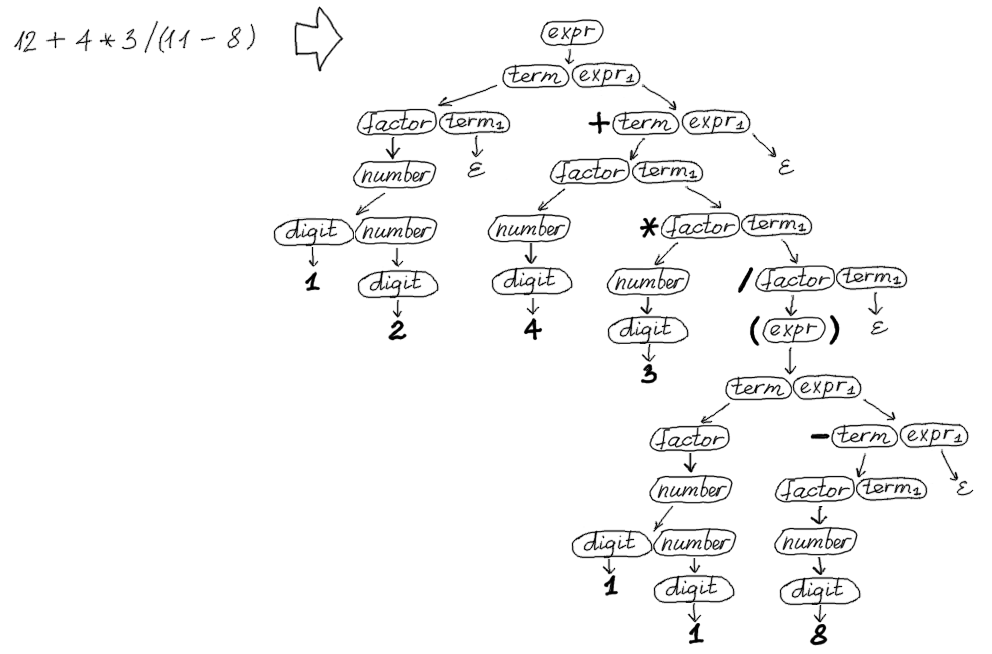
\includegraphics[height=3.5in]{pic/19.png}
\\ \\
Дерево разбора представляет структуру арифметического выражения в точном соответствии с грамматикой.
Это дерево хорошее и правильное, но какое-то оно \emph{слишком детальное}.
Например, чтобы добраться до числа $12$, надо обойти вершины $expr$, $term \ expr_1$, $factor \ term_1$ и $number$,
а потом ещё по кускам собирать само число из цифр, сидящих в вершинах $digit$.
Зачем нам хранить в AST информацию, что число $12$ получилось таким хитрым путём?
Ненужная детализация --- это источник бед. Во-первых, она дурит голову (например,
я размазываю простенький пример на десять страниц, и ты не улавливаешь сути). Во-вторых,
все эти детали надо где-то хранить (для больших выражений потребуется уйма памяти).
В-третьих, обходя огромное дерево, больше шансов где-то сделать ошибку.
\\ \\
Человек представляет себе выражение $12 + 4 * 3 / (11 - 8)$ вот так:
\\ \\
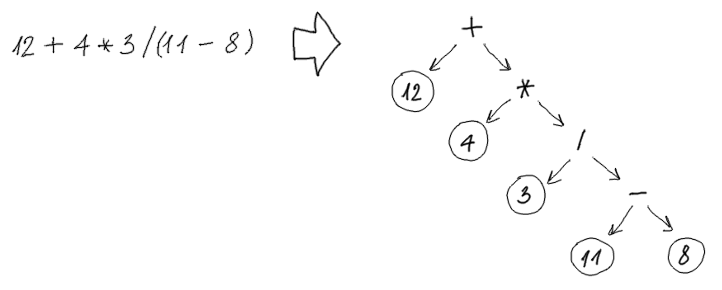
\includegraphics[height=2in]{pic/20.png}
\\ \\
Это дерево отражает структуру выражения ничуть не хуже,
чем дерево разбора, но при этом оно намного проще и компактнее. Почему мы не можем
сделать дерево разбора таким же простым? Дерево разбора зависит только от грамматики.
Чтобы дерево разбора было красивым, нужна другая, красивая грамматика. К несчастью,
красивые грамматики обычно напичканы неоднозначностями, и парсер для них написать
очень трудно или вообще невозможно (кроме того, такие парсеры работают очень медленно).
Наша грамматика некрасивая, потому что она приспособлена для компьютера, а не для человека.
Но никто не мешает нам сделать AST не таким, как дерево разбора.
\\ \\
Итак, в нашем AST будут узлы пяти типов: ``число'', ``плюс'', ``минус'', ``умножить'', ``поделить''.
Узел типа ``число'' всегда будет листом, т.е. у него не будет детей. У остальных типов
узлов будет ровно по два ребёнка: левый и правый операнды. Узлы-операнды могут быть числом
(если тип узла - ``число'') или корнем поддерева (если тип узла --- ``плюс'', ``минус'', ``умножить'' или ``поделить'').
На хаскеле такой тип данных выражается проще некуда:
\begin{verbatim}
data AST
    = Number Int
    | Add AST AST
    | Sub AST AST
    | Mul AST AST
    | Div AST AST
\end{verbatim}
Здесь \texttt{AST} --- тип данных, который мы определяем;
\texttt{Int} --- встроенный хаскельный тип; \texttt{Number},
\texttt{Add}, \texttt{Sub}, \texttt{Mul} и \texttt{Div} ---
функции-конструкторы нашего типа \texttt{AST}. Конструктор может принимать аргументы, как и любая функция:
в нашем случае конструктор \texttt{Number} --- это функция, принимающая один аргумент типа \texttt{Int},
а конструкторы \texttt{Add}, \texttt{Sub}, \texttt{Mul} и \texttt{Div} ---
функции, принимающие по два аргумента типа \texttt{AST}. Определения для этих функций писать не надо:
они настолько очевидные, что компилятор сгенерирует их сам.
Теперь сделаем так, чтоб наш парсер сохранял результаты разбора в структуру AST:
\lstinputlisting[language=C++]{example_recursive_descent/parser4_ast.hs}
Раньше нас не интересовал результат работы парсера: всё наши
функции-парсеры возвращали значение типа \texttt{()}. Теперь каждая функция-парсер возвращает результат
своей работы: функции \texttt{digit} и \texttt{number} возвращают результат типа \texttt{Int},
а остальные --- результат типа \texttt{AST}. Функции \texttt{expr1} и \texttt{term1}
теперь принимают параметр типа \texttt{AST} --- левый операнд. Затем они пытаются распарсить правый операнд,
и если это удаётся, то из двух операндов строится новый \texttt{AST}, а если нет --- возвращается левый
операнд. Функция \texttt{number} теперь принимает один аргумент типа \texttt{Int} --- частично вычисленное число.
\\ \\
В тех местах, где возвращаемое из парсера значение важно, вместо оператора \texttt{>\thinspace >}
используется очень похожий оператор \texttt{>\thinspace >=}. Отличие этих двух операторов в том, что \texttt{>\thinspace >}
игнорирует значение, возвращаемое первым парсером, а \texttt{>\thinspace >=} передаёт это значение
второму парсеру в качестве аргумента. Иногда надо не просто передать значение второму парсеру,
а как-то более хитро его использовать.
Чтобы как-то назвать, \emph{обозначить} это возвращаемое значение, используется синтаксис \emph{лямбда-функции}:
\texttt{\textbackslash <arguments> -> <calculations with arguments>}.
\\ \\
\texttt{deriving (Show)} (строка 9) говорит компилятору, что надо сгенерировать функции для вывода
значений типа \texttt{AST} на экран. Без этого мы не смогли бы распечатать полученный \texttt{AST}
(строка 44).
\\ \\
Если что-то непонятно в этом исходнике --- не переживай. Здесь уже слишком много хаскельного сиснтакса,
чтобы всё сразу было понятно. Я привожу примеры на хаскеле по двум причинам: во-первых, потому что
на хаскеле они короткие и способствуют пониманию алгоритма; во-вторых, чтоб заинтересовать тебя.
\\ \\
Теперь напишем тот же самый парсер на С++. Вот как выглядит структура \texttt{AST} (файл ast.h):
\lstinputlisting[language=C++]{example_lang_proc/ast.h}
В файле ast.cpp находится реализация конструкторов и деструкторов \texttt{AST}:
\lstinputlisting[language=C++]{example_lang_proc/ast.cpp}
Теперь перейдём к самому парсеру. По сути он мало отличается от хаскельного
парсера, хотя и не такой элегантный. На C++ нам надо вручную следить
за продвижением указателя во входной строке, поэтому мы передаём его первым аргументом
во все функции (в хаскеле это неявно делала библиотека Parsec).
Обрати внимание, что указатель везде передаётся \emph{по ссылке}, поэтому все изменения, которые делает с ним \emph{вызываемая}
функция, становятся видны \emph{вызывающей} функции. Вот прототипы
функций-парсеров (parser.h):
\lstinputlisting[language=C++]{example_lang_proc/parser.h}
А вот их реализации (parser.cpp):
\lstinputlisting[language=C++]{example_lang_proc/parser.cpp}
Вот и всё! Парсер готов. Он, конечно, далеко не идеален (в частности, плохо обрабатывает ошибки).
Но больше мы его менять не будем.

\subsubsection{Интерпретатор}
Интерпретатор выглядит до смешного просто. Вот его прототип (файл interpreter.h):
\lstinputlisting[language=C++]{example_lang_proc/interpreter.h}
А вот реализация (файл interpreter.cpp):
\lstinputlisting[language=C++]{example_lang_proc/interpreter.cpp}
Функция \texttt{interpret} определяет тип узла: если это \texttt{NUMBER},
то нужно просто вернуть соответствующее число; иначе нужно рекурсивно вычислить
значение левого и правого операндов и вернуть результат операции над ними.

\subsubsection{Компилятор}
Компилятор структурно не сложнее интерпретатора: он точно так же рекурсивно обходит
\texttt{AST}, только вместо немедленного вычисления генерирует машинные инструкции.
Первым делом надо решить важный вопрос: для какой архитектуры?
\\ \\
Архитектура компьютера --- понятие широкое. Нас интересует \emph{архитектура как набор команд процессора} 
(Instruction Set Architecture, ISA). Можно сделать два совершенно
разных процессора, которые будут понимать один и тот же набор команд. Компилятор не увидит
разницы меду ними: ему всё равно, как процессор устроен физически.
Единственное, что компилятору надо знать --- это какие команды понимает процессор
и насколько эффективно он выполняет конкретную команду. Поэтому, говоря об
архитектуре, я имею в виду набор команд процессора.
\\ \\
Какую архитектуру нам выбрать? В принципе, \emph{любую}. Можно, к примеру, выбрать
исторически первый компьютер и компилировать в машинный код для него. 
Только вот запустить такую программу будет негде, поэтому лучше выбрать 
архитектуру твоего компьютера. Кстати, что это за архитектура?
\\ \\
Это можно узнать несколькими способами. Например, поискать в интернетах спецификацию
этой модели (Lenovo ThinkPad X220i). Привожу её тут полностью (вдруг что полезное узнаешь про свой комп),
но нас интересует только секция ``Processor / Chipset'':

\begin{scriptsize}
\begin{verbatim}
Lenovo ThinkPad X220i

    Processor / Chipset
        CPU                                 Intel Core i3 (2nd Gen) 2310M / 2.1 GHz
        Number of Cores                     Dual-Core
        Cache                               L3 - 3 MB
        64-bit Computing                    Yes
        Chipset                             Mobile Intel QM67 Express
        Features                            Intel Turbo Boost Technology 2.0

    Memory
        Max RAM Supported                   8 GB
        Technology                          DDR3 SDRAM
        Speed                               1333 MHz / PC3-10600
        Form Factor                         SO DIMM 204-pin
        Slots Qty                           2
        Empty Slots                         1

    Storage
        Interface                           Serial ATA-300

    Display
        LCD Backlight Technology            LED backlight
        Widescreen                          Yes
        Image Aspect Ratio                  16:9
        Features                            anti-glare

    Audio & Video
        Graphics Processor                  Intel HD Graphics 3000
        Memory Allocation Technology        Dynamic Video Memory Technology
        Camera                              Yes
        Resolution                          0.92 Megapixel
        Capture Resolutions                 1280 x 720
        Sound                               Stereo speakers , stereo microphone
        Codec                               CX20672
        Compliant Standards                 High Definition Audio

    Input
        Type                                touch-screen
        Features                            spill-resistant

    Communications
        Wireless                            Bluetooth 3.0
        Wireless Controller                 Intel Centrino Wireless-N 1000
        Network Interface                   Gigabit Ethernet

    Wireless Broadband (WWAN)
        Generation                          3G upgradable

    Battery
        Installed Qty                       1
        Max Supported Qty                   2
        Run Time                            8.8 sec

    AC Adapter
        Input                               AC 120/230 V ( 50/60 Hz )
        Output                              65 Watt

    Connections & Expansion
        Slots                               1 x ExpressCard/54 ( 1 free )
        Interfaces                          2 x USB 2.0
                                            PoweredUSB
                                            VGA
                                            DisplayPort
                                            LAN
                                            Headphone/microphone combo jack
                                            Dock
        Memory Card Reader                  3 in 1 ( SD Card, SDHC Card, SDXC Card )

    Software
        Software Included                   ThinkVantage Toolbox
        Microsoft Office Preloaded          Includes a pre-loaded image of select Microsoft Office
                                            suites. Purchase an Office 2010 Product Key Card or
                                            disc to activate preloaded software on this PC.

    Miscellaneous
        Security                            Trusted Platform Module (TPM 1.2) Security Chip,
                                            fingerprint reader
        Features                            Intel Active Management Technology (iAMT)
        Compliant Standards                 RoHS
        Manufacturer Selling Program        TopSeller

    Dimensions & Weight
        Width                               12 in
        Depth                               9 in
        Height                              1.2 in
        Weight                              3.7 lbs

    Environmental Standards
        ENERGY STAR Qualified               Yes

    Sustainability
        ENERGY STAR Qualified               Yes
        Greenpeace policy rating (Nov 2011) 3.8

    General
        Manufacturer                        Lenovo
\end{verbatim}
\end{scriptsize}
Видно, что процессор у тебя --- Intel Core i3, двухъядерный и 64-разрядный. Описание
архитектуры этого процессора найти несложно.
\\ \\
Другой, линуксоспецифичный, способ --- выполнить одну из
команд \texttt{arch}, \texttt{uname -m}, \texttt{lscpu}, \texttt{cat /proc/cpuinfo} или ещё какую-нибудь.
Команды \texttt{arch} и \texttt{uname -m} просто бесхитростно пишут название архитектуры (эти команды идентичны).
Команда \texttt{lscpu} кроме архитектуры выводит больше информации о процессоре,
а команда \texttt{cat /proc/cpuinfo} вываливает ту же информацию, только
более размазанно.
\\ \\
Но что, если ты не знаешь модель (нашла компьютер в канаве), и операционная система на нём
очень глупая? Можно попробовать расковырять исполняемый файл какой-нибудь программы, которая запускается
на этом компьютере. Попытаться понять, что там за инструкции (не самый лёгкий способ).
Можно пытаться запустить программы для разных архитектур (пока компьютер не взорвётся).
Если компьютер после этих экспериментов больше не включается, можно расковырять его внутренности.
В общем, есть способы.
\\ \\
У меня есть основания предполагать, что архитектура твоего компьютера --- x86.
Как и моего, и вообще, большинства ноутбуков и десктопов, которые ты видишь.
Про эту архитектуру написано много, и я только вкратце упомяну только самое основное.
\begin{itemize}
\item \textbf{Память: оперативная, регистровая, кэш.}
\\
Процессор работает с какими-то \emph{данными}: команды могут принимать на вход \emph{операнды}
и возвращать \emph{результат}. Эти данные надо где-то хранить. Можно хранить их в оперативной памяти,
но это очень неэффективно: доступ к ней занимает на порядки больше времени, чем выполнение команды.
Поэтому у процессора есть свой маленький кусок сверхбыстрой памяти --- \emph{регистры}.
Понятно, что иногда нужно обмениваться данными между регистрами и памятью: загружать новые данные и выгружать старые.
Поэтому должны быть как минимум две команды работы с памятью: загрузка и выгрузка (load/store).
Обычно в процессоре есть ещё несколько уровней \emph{кэш-памяти}, переходной между регистровой и оперативной.
Программист не управляет кэшами напрямую --- процессор сам решает, какие данные лучше
поместить в кэш. Есть несколько команд, позволяющих влиять на кэширование данных.
\\ \\
Примерно так выглядят регистры процессора x86-64:
\\
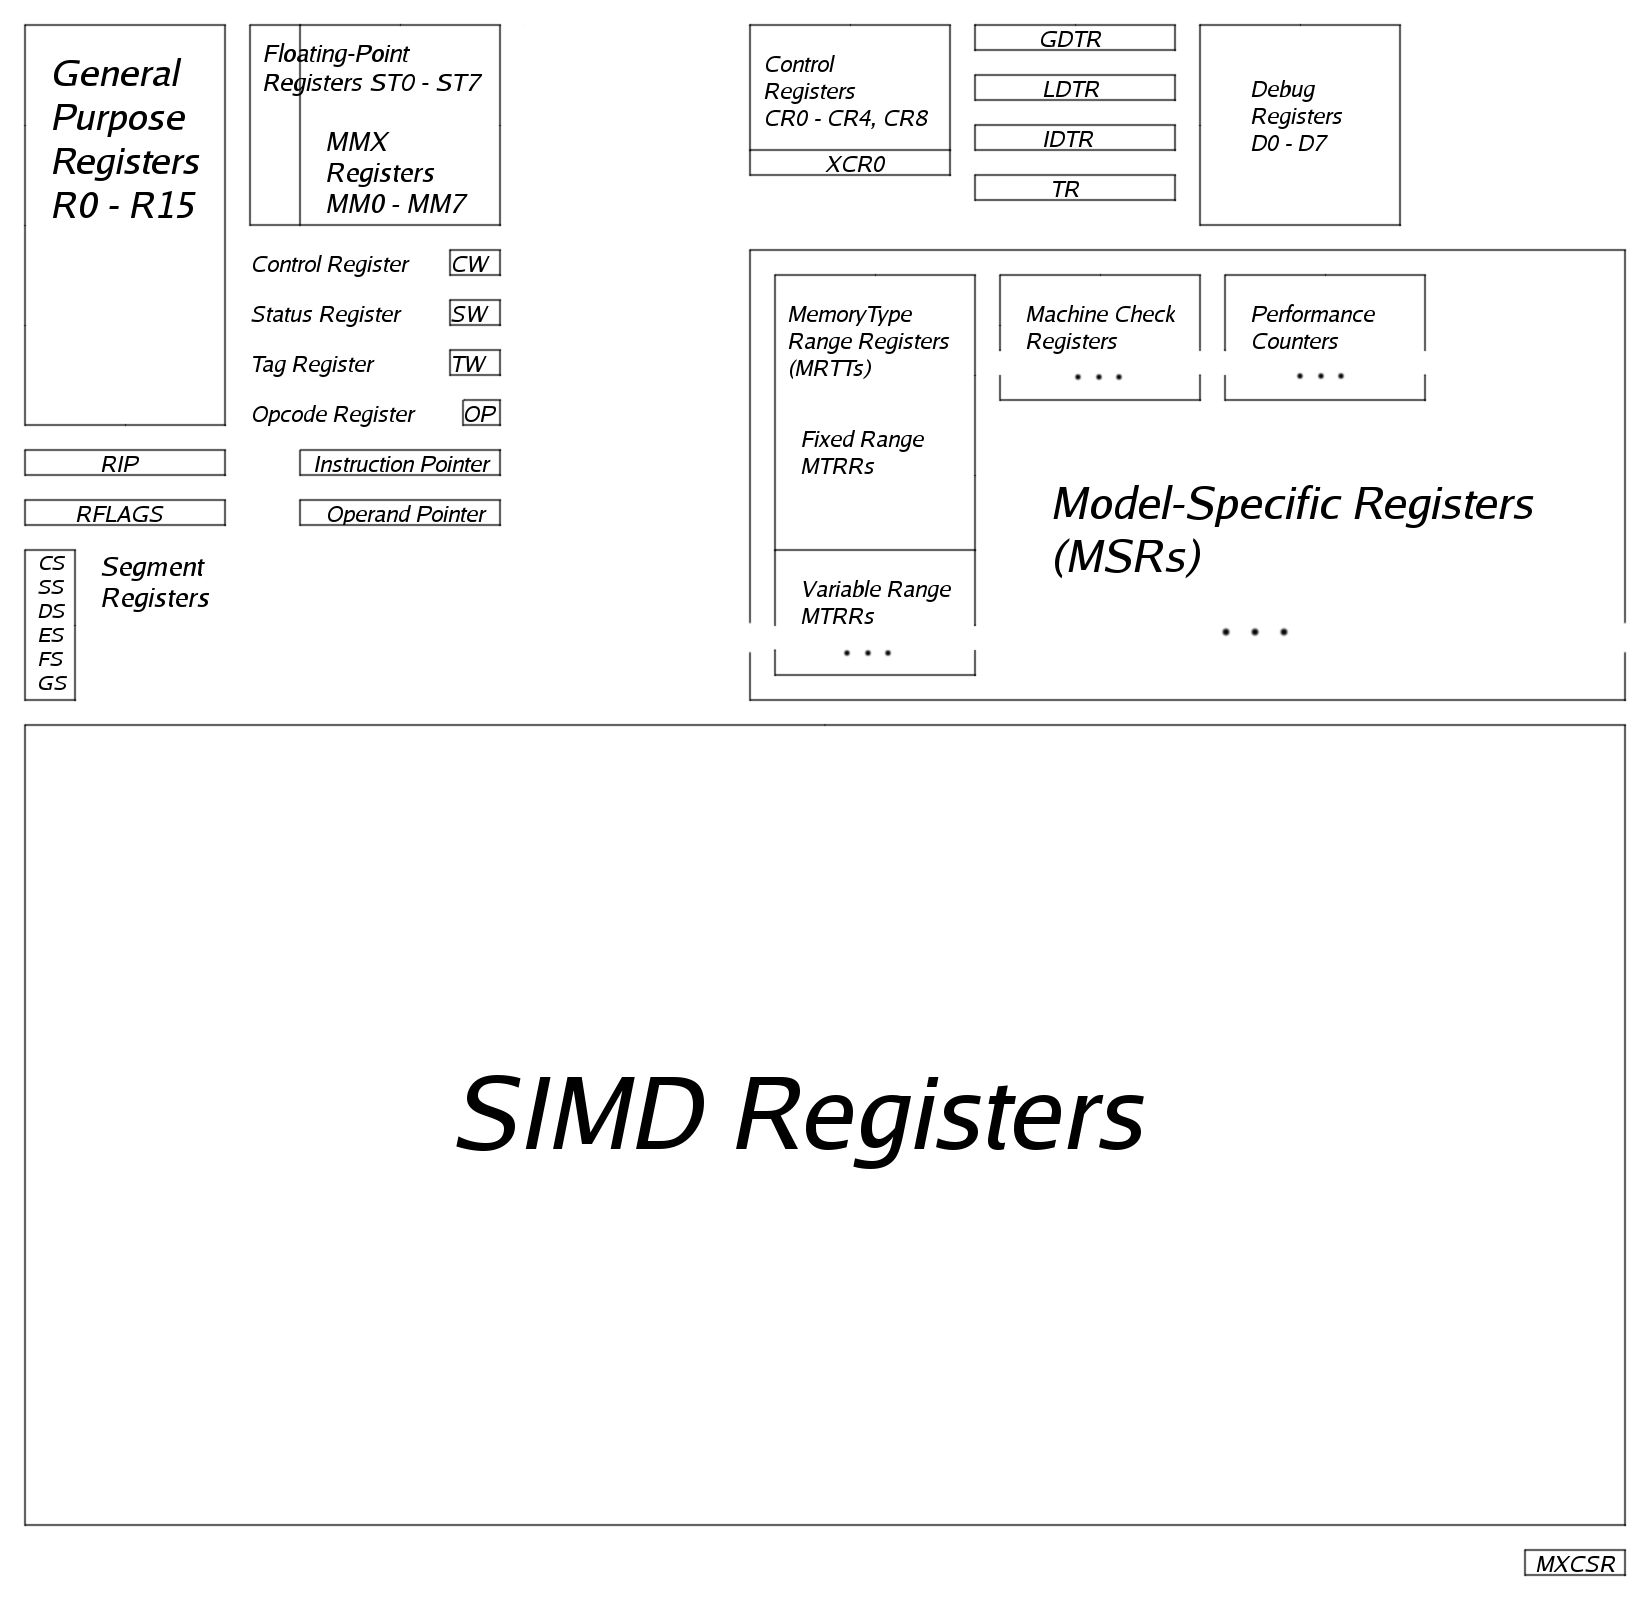
\includegraphics[width=6in]{pic/registers.png}
\\
    \begin{enumerate}
    \item Application registers
        \begin{enumerate}
        \item general purpose registers: RAX, RBX, RCX, RDX, RDI, RSI, RBP, RSP и R8 - R15
        \item segment registers CS, SS, DS, ES, FS, GS
        \item instruction pointer register RIP
        \item flag register RFLAGS
        \item FPU registers ST0 - ST7, control registers CW, SW, TW, FP\_OPC, FP\_IP, FP\_DP
        \item SIMD registers: MMX, SSE, AVX, control/status register MXCSR
        \end{enumerate}
    \item System registers
        \begin{enumerate}
        \item control registers CR0 - CR4, CR8, XCR0
        \item descriptor table registers GDTR, IDTR, LDTR, TR
        \item debug registers DR0 - DR15
        \item memory type range registers (MTRRs)
        \item machine specific registers (MSRs)
        \item machine check registers
        \end{enumerate}
    \end{enumerate}
В мануале ``Intel 64 and IA-32 Architectures Software Developer's Manual'' можно найти
описание всех регистров, для чего они нужны и как их использовать. Системные регистры описаны
в третьем томе (так что тебе придётся прочитать его, когда надумаешь писать операционную систему ;)).
В компиляторе мы будем в явном виде использовать только несколько регистров общего назначения,
да и то в основном их младшие 32 бита.
\\ \\
Регистры общего назначения:
\\
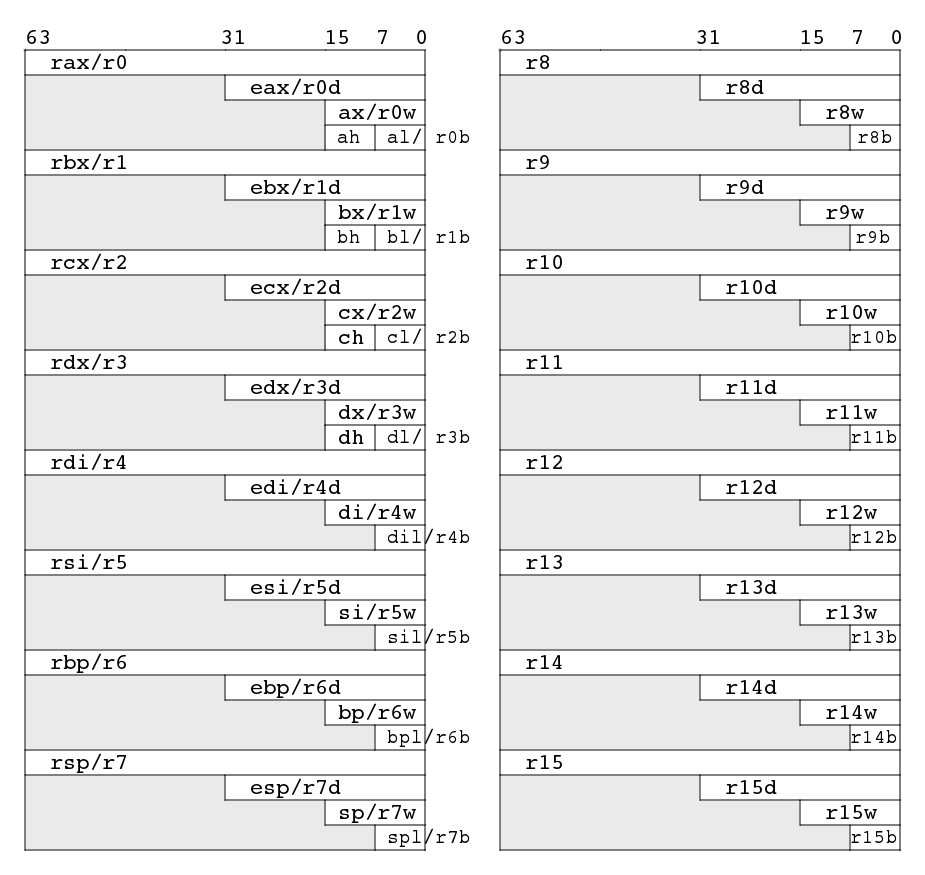
\includegraphics[height=4in]{pic/registers_general_purpose.png}
\item \textbf{CISC и RISC.}
\\
На ассемблере программировать сложно: очень уж большой разрыв между высокоуровневыми идеями
в человеческой голве и низкоуровневыми машинными инструкциями.
В программах часто повторяются одни и те же последовательности команд, выполняющие какую-то конкретную задачу.
Естественная мысль --- заменить такие последовательности одной командой.
(Это можно сделать по-разному.
Можно попросту зашить новые сложные команды в процессор, но это сильно усложнит и специализирует процессор.
Поэтому обычно идут другим путём: сложные команды составляют из простых в виде \emph{микропрограмм}.
В процессор встраивают \emph{интерпретатор микрокода}, который раскладывает микропрограммы на простые команды.
Чтобы добавить или поменять команду, нужно просто сохранить её микрокод в специальную область памяти.
С одной стороны, такой подход позволяет внутреннему процессору оставаться простым.
С другой стороны, появляется невероятная гибкость: добавляя новые команды, можно одну и ту же машину
превратить в утюг или кассовый аппарат.
Теоретически изменять микрокод может кто-угодно, но некоторые жадные производители железа не хотят делиться.)
Как бы там ни было, появление сложных команд приводит к сильному расслоению команд по времени выполнения: простые команды
выполняются очень быстро, а сложные очень долго. (В частности из-за того, что появляется много команд, работающих с памятью.)
Такие архитектуры называются CISC (Complex Instruction Set Computer).
\\ \\
Второй подход --- RISC (Reduced Instruction Set Computer) --- возник, когда стало ясно, что часто ассемблерная программа из простых команд
более эффективна, чем сложная команда. Между простыми командами легче отслеживать \emph{зависимости},
поэтому часто их удаётся переставлять местами и выполнять параллельно.
Основная идея RISC-архитектуры --- сделать так, чтобы почти все команды выполнялись быстро (за один или несколько тактов процессора).
Поскольку доступ к памяти занимает много времени, оставляют только две команды работы с памятью: загузка и выгрузка.
\\ \\
Неправильно думать, что CISC-архитектуры сложные, а RISC-архитектуры простые. Слова ``complex'' и ``reduced''
относятся к скорости выполения команд, а не к их многообразию. Есть очень простые CISC-ахитектуры
и очень сложные RISC-архитектуры. Многие архитектуры смешивают в себе RISC и CISC черты.
Об этом всём хорошо написано в статье ``Processor Architectures. RISC-CISC-Harvard-Von Neumann''. :)
\\ \\
x86 --- пример очень сложной CISC-архитектуры.
Её сложность ты можешь на глаз оценить по размеру мануала ``Intel 64 and IA-32 Architectures Software Developer's Manual''.
\item \textbf{Кодирование команд.}
\\
Команды в x86 кодируются байтовыми последовательностями разной длины (от 1 до 15 байт).
Каждя команда начинается с \emph{опкода}, который занимает от одного до трёх байт.
У каждой команды свой, уникальный опкод (поэтому её нельзя спутать с другой командой).
После опкода могут быть другие, командо-специфичные байты. В них закодированиы
операнды: номера регистров, адреса в памяти или \emph{непосредственные операнды}
(т.е. константы, зашитые прямо в инструкцию). Детальное описание всех команд x86
ты найдёшь в мануале ``Intel 64 and IA-32 Architectures Software Developer's Manual'',
тома 2a и 2b.
\item \textbf{Разрядность.}
\\
Под разрядностью понимается, сколько битов влазит в регистр и какой размер адреса в памяти.
Если регистр $N$-разрядный, то максимальное беззнаковое целое число, которое в него влезет, --- $2^N$.
Если адрес $N$-разрядный, то максимальный объём памяти, который можно адресовать в программе, --- $2^N$ бит.
Разрядность обычно кратна восьми (т.е. числу бит в байте), но не обязательно.
У архитектуры x86 есть 16-разрядный, 32-разрядный и 64-разрядный варианты (каждый следующий вариант
совместим с предыдущими, т.е. понимает программы для предыдущих). У твоего ноутбука архитектура
x86-64.
\item \textbf{Порядок байт.}
\\
Память обычно адресуется побайтно.
Понятие \emph{endianness} означает порядок, в котором многобайтные значения хранятся в памяти.
Big-endian --- байты храняться от старших к младшим (так же, как мы записываем число на бумажке).
Little-endian --- байты хранятся от младших к старшим (задом наперёд).
\\
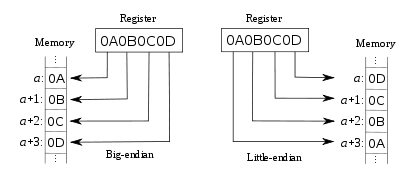
\includegraphics[height=1.75in]{pic/22.png}
\\
Архитектура x86-64 --- little-endian.
\end{itemize}
Теперь пора задуматься, как будет выглядеть наша программа. Для начала возьмём очень простую
программу: $1 + 2$. Команда для сложения --- \texttt{ADD}.
Откроем мануал ``Intel 64 and IA-32 Architectures Software Developer's Manual'', том 2a,
на описании команды \texttt{ADD}:
\\ \\
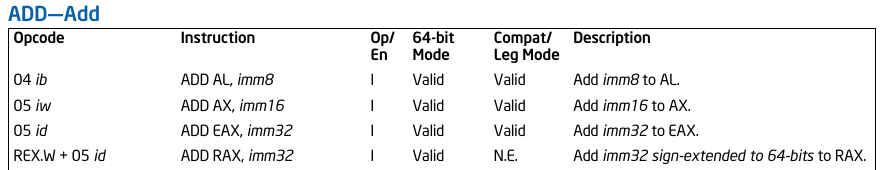
\includegraphics[width=6in]{pic/21a.png}
\\
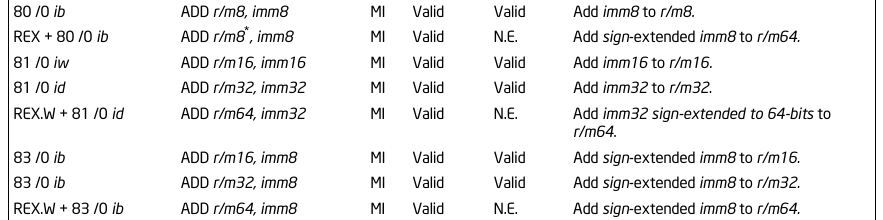
\includegraphics[width=6in]{pic/21b.png}
\\
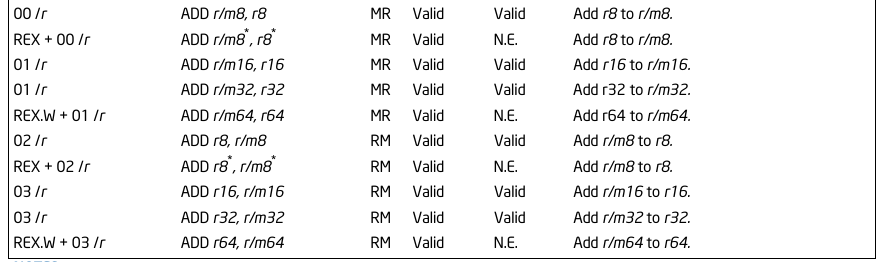
\includegraphics[width=6in]{pic/21c.png}
\\ \\
О-хо-хо! На одно только описание разных видов команды \texttt{ADD} ушла целая страница.







\lstinputlisting[language=C++]{example_lang_proc/compiler.h}
\lstinputlisting[language=C++]{example_lang_proc/compiler.cpp}
\subsubsection{Виртуальная машина: байткод}
\lstinputlisting[language=C++]{example_lang_proc/vm_bytecode.cpp}
\lstinputlisting[language=C++]{example_lang_proc/vm_bytecode.h}
\subsubsection{Виртуальная машина: интерпретатор байткода}
\lstinputlisting[language=C++]{example_lang_proc/vm_run.cpp}
\lstinputlisting[language=C++]{example_lang_proc/vm_run.h}
\subsubsection{Виртуальная машина: JIT-компилятор байткода}
\lstinputlisting[language=C++]{example_lang_proc/vm_jit.cpp}
\lstinputlisting[language=C++]{example_lang_proc/vm_jit.h}
\subsection{Как всё в реальной жизни}
...
\section{Синтаксический анализ}
...
\chapter{Основы языков программирования}
...
\section{Синтаксис и семантика}
...
\section{Структура языка}
...
\subsection{Примитивы}
...
\subsection{Переменные}
...
\subsection{Типы}
...
\subsection{Выражения}
...
\subsection{Утверждения}
...
\subsection{Управляющие конструкции}
...
\subsection{Функции}
...
\subsection{Сложные типы и отношения между типами}
...
\subsection{Области видимости}
...
\subsection{Полиморфизм (параметрический, ad-hoc, полиморфизм подтипов)}
...
\subsection{Расширяемость}
...
\section{Язык в действии}
...
\subsection{Выразительная сила языка (тьюринг-полнота)}
...
\subsection{Математическая модель вычислений}
...
\subsection{Статическое и динамическое в языке}
...
\subsection{Управление памятью}
...
\subsection{Параллельные вычисления}
...
\subsection{Динамическая генерация кода}
...
\subsection{Рантайм и стандартная библиотека}
...
\section{Что важно для программиста}
...

\end{document}